\section{Cronograma e Disciplinas}

Este projeto visa ser desenvolvido no Laboratório de Transmissão e Tecnologia do Calor (LTTC) do Programa de Engenharia Mecânica da Coppe (PEM/COPPE). 
Tal laboratório dispõe de uma ampla infraestrutura, 
além de recursos computacionais de última geração, 
voltada a projetos de pesquisa, desenvolvimento e inovação
em termociências, em diversas linhas, 
inclusive em simulações com o uso de métodos numéricos \cite{lttccoppe}. 

\bigskip
Para este projeto as seguintes metas serão propostas, conforme apresentado no cronograma a seguir:

\begin{enumerate}

\item No primeiro ano, concluir 100\% da carga horária do curso com CRA superior a 2.0 e ser aprovador nas Fases I e II do Exame de Qualificação;

\item No segundo ano, concluir a Revisão Bibliográfica e iniciar a implementação do Código Numérico;

\item No terceiro ano, concluir a implementação e validação do código numérico;

\item No quarto ano, finalizar as simulações do problema proposto, publicar os resultados em canais de alto impacto e apresentar a Tese de Doutorado.

\hspace{-1.2cm}
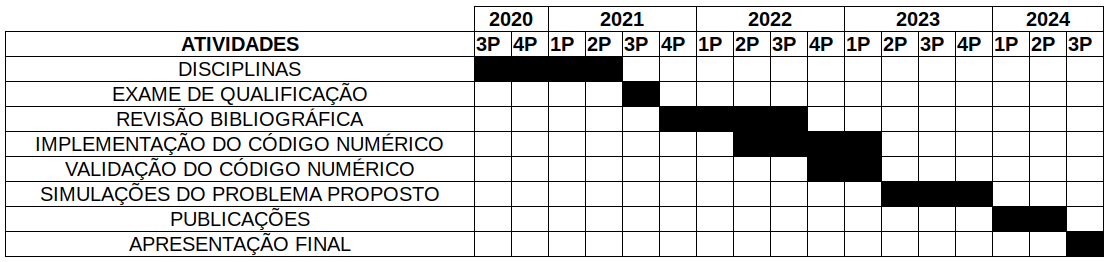
\includegraphics[scale=0.44]{figure/cronograma.png}

\end{enumerate}

\bigskip
As disciplinas a serem realizadas são:

\begin{enumerate}
\item COM774 - Métodos Matemáticos; 
\item COM719 - Mecânica do Contínuo;
\item COM710 - Fundamentos da Mecânica dos Fluidos;
\item COM825 - Escoamento Bifásico;
\item COM795 - Análise Numérica;
\item COM737 - Geração Numérica de Malhas;
\end{enumerate}
